% !TeX encoding = UTF-8
% !TeX spellcheck = fr_FR
% !TeX root = ../mythesis.tex
% !TeX program = pdflatex (build)
%%% TeXmaker : no 'magic comments' but set Root with Options > Set as master file
\graphicspath{{./}{./fig/}{./chap_stimulated_hawking/fig/}}

\chapter{Experimental observation of stimulated Hawking radiation in a polariton quantum fluid}
\label{chap:stimulated_hawking}



In the previous chapter, we demonstrated the experimental realization of a transcritical flow in a polariton quantum fluid through precise optical pump shaping. This allowed us to engineer the fluid's density and velocity profiles to form a transcritical region, a key ingredient for the emergence of a sonic horizon. Additionally, we presented experimental evidence of negative-energy modes in this region, confirming the necessary conditions for the observation of the Hawking effect.

Building on these achievements, this chapter focuses on the experimental observation of stimulated Hawking radiation in a polariton fluid. Stimulated emission provides a controlled way to probe the Hawking effect by injecting a coherent state into the upstream region and measuring its scattering into outgoing modes. This approach allows us to directly study the amplification of positive-energy modes and the role of negative-energy modes in the transcritical region.
The experimental realization of stimulated Hawking radiation involves several key steps. First, we describe the setup used to inject coherent states into the polariton fluid and the techniques employed to measure the outgoing modes. 
Next, we detail the partial reconstruction of the scattering matrix, which encodes the mixing of positive- and negative-energy modes and provides direct evidence of energy amplification.
 Finally, we present the results of these measurements, discuss the agreement with theoretical predictions and the robustness of the stimulated Hawking effect.
The results presented in this chapter not only validate the theoretical predictions of stimulated emission but also establish a pathway toward the observation of spontaneous Hawking radiation. By leveraging the unique properties of polariton fluids, this work demonstrates the potential of these systems as a platform for exploring fundamental aspects of quantum field theory in curved spacetime and beyond.


\begin{figure}[htbp]
    \centering
    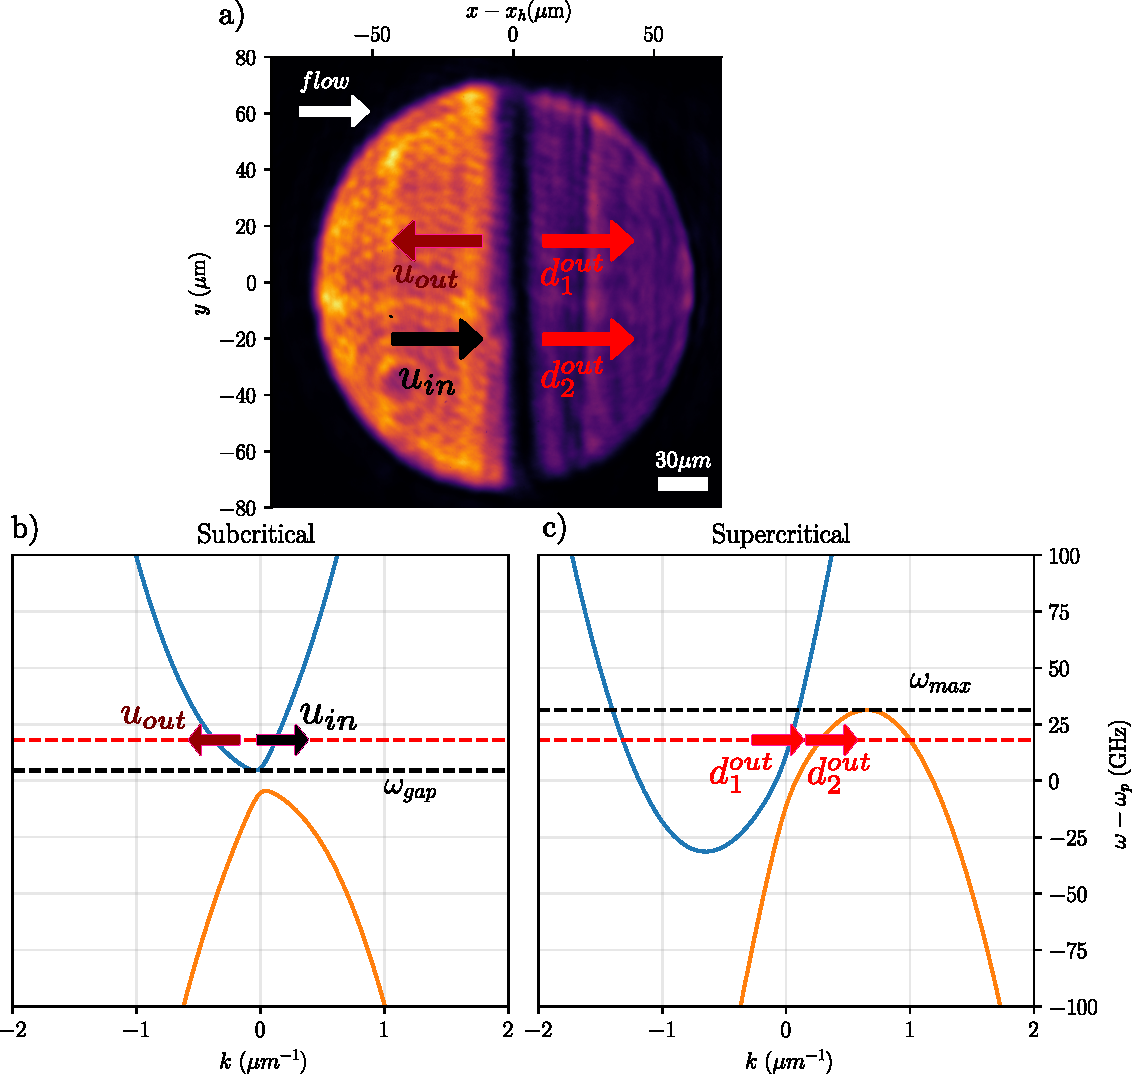
\includegraphics[width=1\textwidth]{chap_stimulated_hawking/fig/typical_dens_2D.pdf}
    \caption{\textbf{a)} Real space image of a transcritical flow of polaritons with detuning $\delta(0)=29 GHz$ and wavevectors $k_u=0.2 \mu m^{-1}$ and $k_d=0.6\mu m^{-1}$. The black arrow represents the impinging mode $u_{in}$ while the blue arrows represent the outgoing modes $u_{out}$, $d_1^{out}$ and $d_2^{out}$. The direction
    of the arrow reflects the sign of the group velocity of each mode.
    \textbf{b)} Typical Bogoliubov dispersion relation in the upstream subcritical region. The arrows correspond to the modes displayed on the left side of \textbf{a)}. 
    \textbf{c)} Typical Bogoliubov dispersion relation in the downstream supercritical region. The arrows correspond to the modes displayed on the right side of \textbf{a)}}
    \label{fig:typical_dens_2D}
\end{figure}


\section{Interferometric measurement of the scattering matrix }
\label{sec:principle_measurement}

We aim at solving the scattering problem of a coherent state injected in the upstream region impinging on the horizon. Doing so, it is possible
to partially reconstruct the scattering matrix. This approach is complementary of what has already been done in other works in which 
the stimulating field was coming from the transcritical region. ???????? 

\subsection{Challenges of the measurement}


Let us take a transcritical flow of polaritons with typical density profile shown in \autoref{fig:typical_dens_2D} \textbf{a)}. The bright
region on the left correspond to the upstream subcritical region while the other side of the interface is the transcritical region. Typical spectra corresponding to each region are shown in \textbf{b)} and \textbf{c)}.
The previous chapter made clear that it is possible to locally excite the Bogoliubov dispersion by shinning a weak probe laser at the right couple $(\omega, k)$. Consider then a coherent state
$\ket{\alpha_{in}}$ in the $u_{in}$ mode of \textbf{b)} that is, an upstream mode impinging on the interface. If its frequency $\omega_{in}$ is within $[\omega_{gap}, \omega_{max}]$ we expect to measure one reflected mode $u_{out}$ and two transmitted modes $d_1^{out}$ and $d_2^{out}$. The latter is the negative
energy mode responsible for Hawking radiation. Each of this mode has a different wavevector $k_i$.

\bigskip


Experimentally, this situation corresponds to four distinct optical signals exiting the sample at different angles, or equivalently, to four spatially separated spots in the Fourier plane of the cavity. To illustrate the inherent challenges associated with such measurements, we present in \autoref{fig:bh_k_space} \textbf{b)} the typical expected locations of the scattered signals in the Fourier plane corresponding to the fluid configuration of \autoref{fig:typical_dens_2D} \textbf{a)}. The two bright spots correspond to the regions of the fluid characterized by the wavevectors \(k_u\) and \(k_d\). Two principal experimental challenges can be identified. 

First, the expected position of the mode \(d_1^{\text{out}}\) nearly coincides with the pump signal in the downstream region. Since the probe intensity must remain at least two orders of magnitude lower than that of the pump to preserve the perturbative regime, the resulting signal-to-noise ratio is extremely low. Consequently, a direct measurement of the \(d_1^{\text{out}}\) mode becomes unfeasible.

Second, in addition to the desired signals at frequency \(\omega_{\text{in}}\), all modes are subject to four-wave mixing processes due to nonlinear interactions with the pumped polaritons. As a result, depending on the fluid parameters, the conjugated modes generated by these interactions may spatially overlap with the reflected or transmitted modes. For example, as illustrated in \autoref{fig:bh_k_space}, the conjugate of the injected mode \(u_{\text{in}}\) appears at the same location in momentum space as the reflected mode \(u_{\text{out}}\). Consequently, placing a pinhole at this position does not permit one to distinguish between the two contributions.

The central challenge of this measurement is thus to detect weak signals on top of a strong background while ensuring that these signals originate from genuine transmission and reflection at the interface --rather than from spurious scattering events or nonlinear mixing. Therefore, the critical experimental objective is to optimize the signal-to-noise ratio, where “noise” refers to all undesired signals. This is achieved by acting on two main experimental parameters:


\begin{figure}
    \centering
    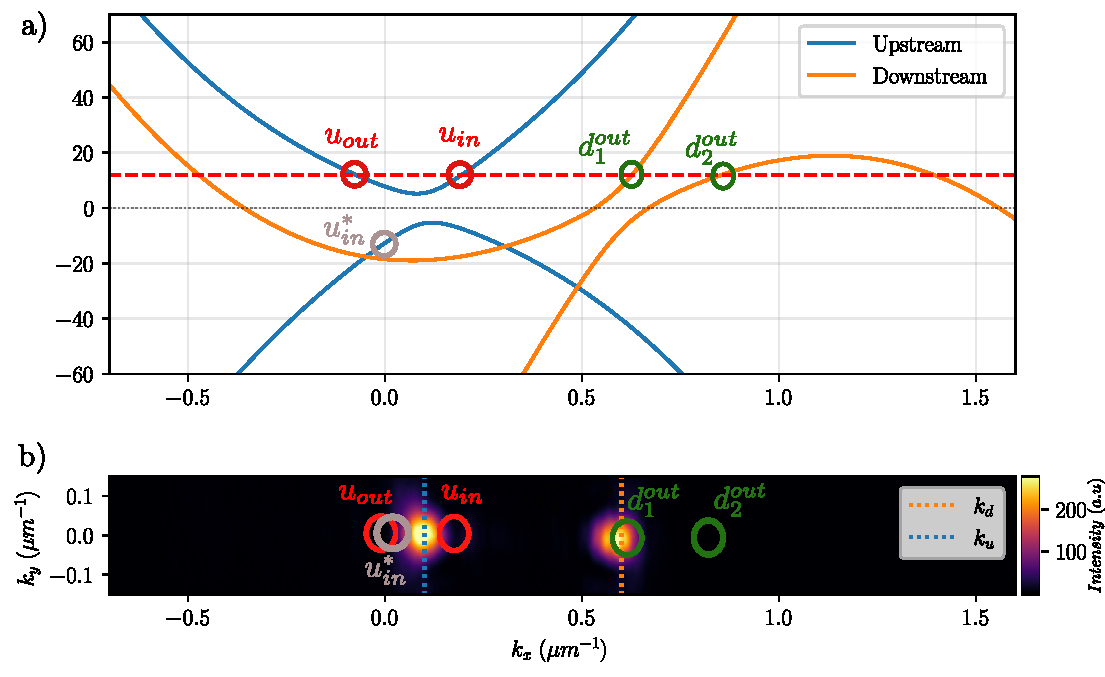
\includegraphics[width=1\textwidth]{chap_stimulated_hawking/fig/bh_k_space.pdf}
    \caption{\textbf{a)} Analytical Bogoliubov dispersion of both regions calculated with the parameters of the fluid of \autoref{fig:typical_dens_2D} \textbf{a)}. To reflects what happen in practice, the two dispersion are plotted in the same graph as a function of the wavevector in the laboratory frame $k$. The upstream dispersion
    is centered at $k_u$ while the downstream one is centered at $k_d$. The red dashed line corresponds to the energy of the injected mode. The wavevectors of the reflected-transmitted is obtained 
    at the intersections of this line with the Bogoliubov branches and reported in the momentum space \textbf{b)}.The red (resp. green) circle represent the expected location 
    of the upstream (resp. downstream) modes. Finally, the grey circle represent the conjugated of the injected signal resulting from four wave mixing. \textbf{b)} Momentum space of \autoref{fig:typical_dens_2D} \textbf{a)} : the two bright spots correspond to the two region of the fluid with wavevectors $k_u$ and $k_d$. The colored circle
    are reported from \textbf{a)}.}
    \label{fig:bh_k_space}
\end{figure}

\begin{itemize}
    \item \textbf{Enhancement of the signal}: As discussed in the previous chapter, this can be accomplished by increasing the steepness of the horizon.
    \item \textbf{Suppression of the pump background}: The photonic nature of the system allows us to exploit two key properties of ligh --polarization and coherence. Polarization filtering can be applied in the detection path, while coherence enables the use of interferometric techniques, as will be detailed in the following section.
\end{itemize}

\textbf{Electronic filtering.} One possible strategy to suppress the pump background is inspired by the method used to measure the excitation spectrum in the previous chapter. By modulating the probe beam intensity at a frequency \(\omega_{\text{mod}}\) accessible in the electronic domain, the signal can later be demodulated, isolating the component arising from the probe-induced excitation. However, in the current context, what previously served as an advantage becomes a limitation. Indeed, the four-wave mixing signals also carry the modulation, thus failing to resolve the overlap problem discussed above. To overcome this, we turn to the optical domain, specifically to interference-based detection schemes.

\subsection{Interferometric reconstruction of the Fluctuation Field}

The measurement is based on the same interferometric technique previously employed to reconstruct the mean field.
 The key distinction here is that the method is now applied to the probe field instead. Although this may appear to be a minor adjustment, it represents a significant conceptual shift that enables a comprehensive characterization of the fluctuations. 
Before detailing its experimental implementation in the context of the scattering problem, we first examine the insights that such a measurement can provide.

\bigskip

We again consider the generic situation presented above namely, a coherent state injected in the upstream region. The full optical field transmitted through
the sample can is composed of :

\begin{itemize}
    \item The mean field $\psi_0$ oscillating at the pump frequency $\omega_p$.
    \item The fluctuation field oscillating at the probe frequency $\omega_{in}$ resulting from the scattering of $u_{in}$ on the interface.
    \item The conjugated field oscillating at the opposite of the probe frequency $-\omega_{in}$ resulting from the four wave mixing of each $+\omega_{in}$ mode with the pump. 
\end{itemize}


\begin{figure}
    \centering
    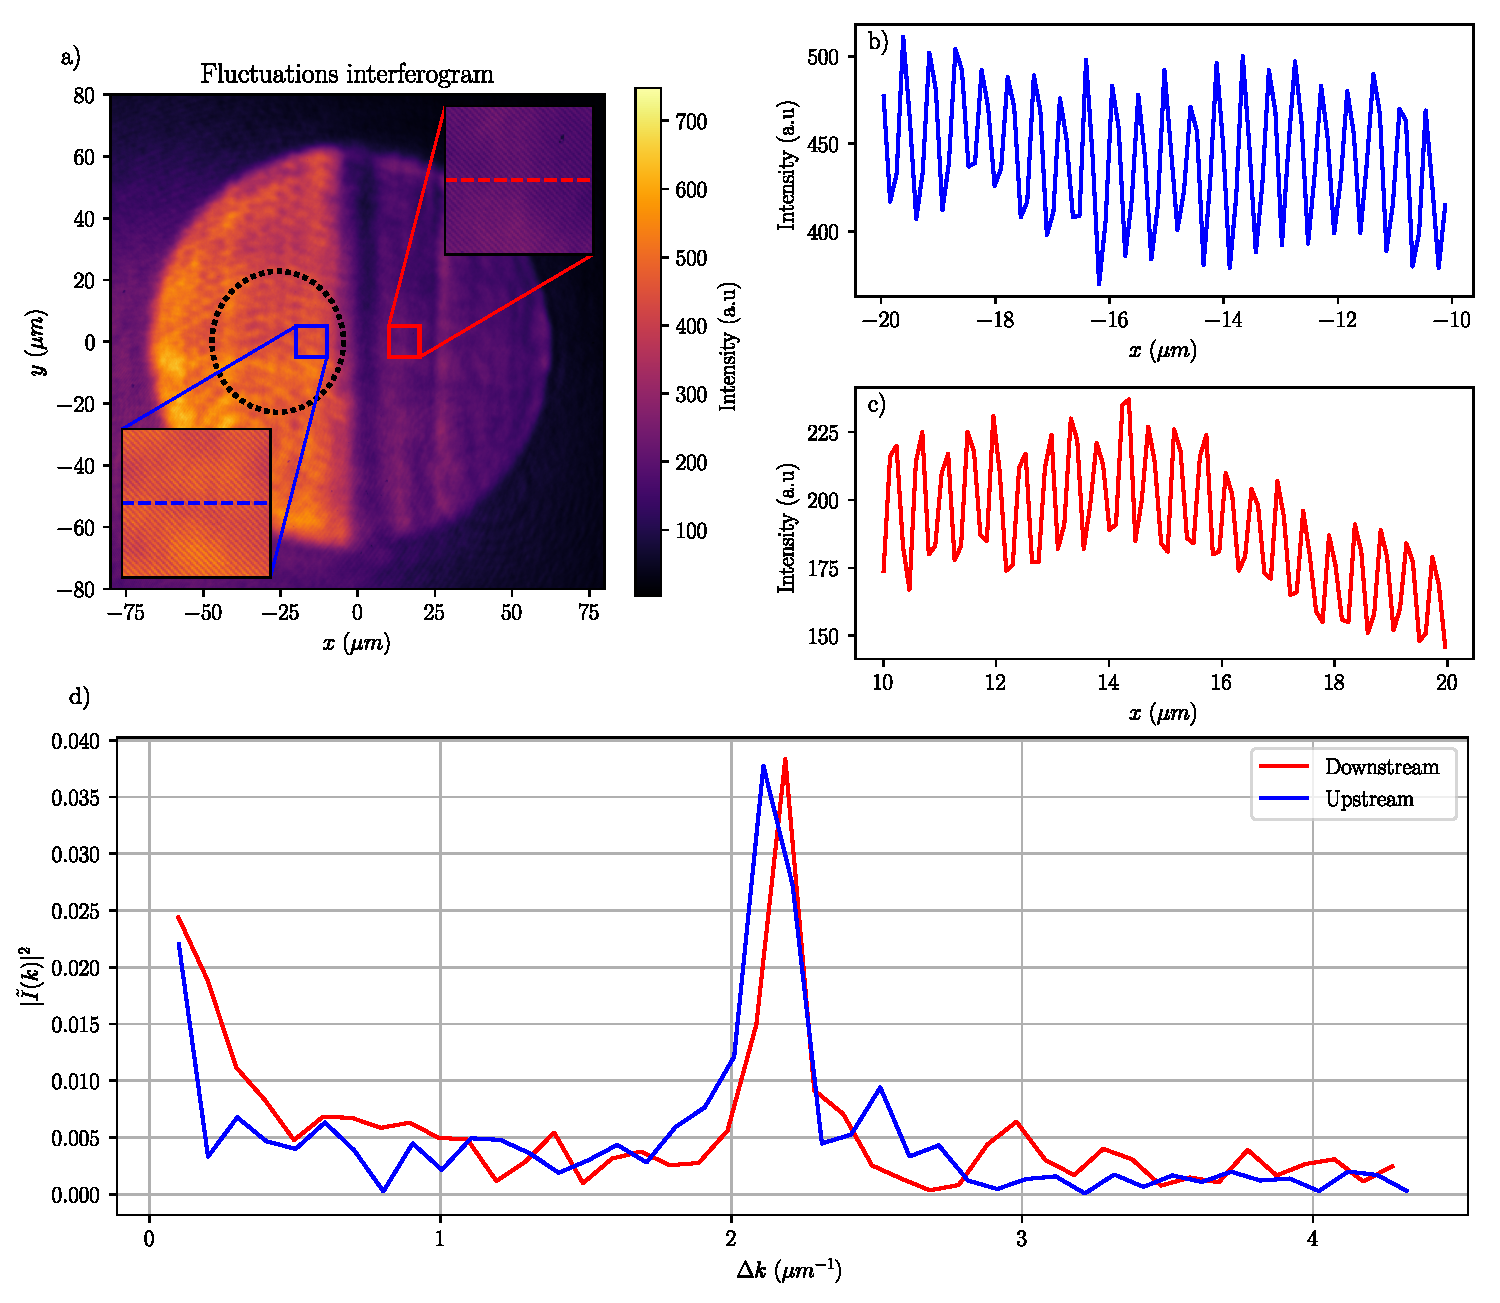
\includegraphics[width=1\textwidth]{chap_stimulated_hawking/fig/interferogram_fluctuations.pdf}
    \caption{\textbf{a)} Interferogram resulting from the supersposition of \autoref{fig:typical_dens_2D} \textbf{a)} and a reference beam from the probe laser. The black dashed circle
    represent the injected probe location. The red inset (resp. blue) is a zoom on the upstream (resp. downstream) region near the interface. 
    \textbf{b)} Cut of the interferogram along the red dashed line of the red inset. 
    \textbf{c)} Cut of the interferogram along the blue dashed line of the blue inset. 
    \textbf{d)} Fourier transforms of the cuts \textbf{b)} and \textbf{c)}. The blue curve corresponds to the upstream region with spatial frequency $\Delta k_u\approx\SI{2.11}{\per \micro \meter}$. The red curve corresponds to the downstream region with spatial frequency $\Delta k_d= \SI{2.19}{\per \micro \meter}$. 
     }
    \label{fig:interferogram_fluctuation}
\end{figure}


When the probe field is superimposed with a phase reference beam at the probe frequency—obtained as a pick-off from the probe laser—the only components that generate interference fringes are those oscillating at \(+\omega_{\text{in}}\). 
Each scattered mode is characterized by a distinct wavevector \(k_i\), leading to a unique spatial frequency in the resulting interferogram.
As an illustrative example, \autoref{fig:interferogram_fluctuation}~\textbf{a)} displays two regions of such an interferogram.
 The first lies within the probe injection area, where the fringe spacing is inversely proportional to \(\abs{\Delta k}\), with \(\Delta k = k_{u_{\text{in}}} - k_{\text{ref}}\) denoting the wavevector mismatch between the injected mode and the reference beam. 
 The second region is located downstream, beyond the probe injection area. The mere presence of interference fringes in this region already confirms that the injected mode has propagated through the interface, while the fringe spacing provides direct information about the wavevector of the transmitted mode.

This interpretation is supported by the spatial Fourier transforms of the two regions, shown in \textbf{d)}. The low-\(\Delta k\) peak corresponds to the continuous background signal—primarily the pump field and the conjugated modes at \(-\omega_{\text{in}}\)—which do not interfere with the reference beam. The central peaks represent the spatial frequencies of the propagating components in each region. Notably, the downstream region exhibits a higher wavevector, consistent with the scattering picture.

This preliminary analysis already highlights the power of the technique. By applying numerical masks at different spatial locations, one can selectively extract the Fourier components of the fluctuations. Put more generally, a single interferogram enables full reconstruction of the fluctuation field at the frequency of the injected perturbation. As a result, this method proves particularly well-suited for addressing the scattering problem, as it inherently overcomes all the challenges previously outlined :



\begin{itemize}
    \item Conjugated modes and background contributions from the pump are inherently filtered out, as they do not interfere with the reference beam and therefore do not generate fringes.
    \item Each scattered mode gives rise to a distinct spatial frequency in the interferogram, enabling their individual identification and selective extraction.
    \item The interference with the coherent reference beam enhances the signal-to-noise ratio, thereby facilitating the detection of weak scattered components.
\end{itemize}


The interferometric technique outlined above provides a powerful framework for reconstructing the fluctuation field and isolating the scattered modes.
 By leveraging the distinct spatial frequencies of the scattered components and filtering out unwanted contributions, this method enables a precise characterization of the scattering process. In the following section, we detail the experimental implementation of this approach, focusing on the setup and procedures required to reconstruct the scattering matrix and extract the key parameters governing the stimulated Hawking effect.

 \section{Experimental implementation}
 The experiment is conducted in the same microcavity as in the previous chapter, operating at the same working point (C5-D6) and using an identical optical setup. 
 However, whereas the previous measurements focused on characterizing the fluid's excitation spectrum, the present objective is to detect the scattered signals generated at the horizon interface. 
 To this end, we first investigate configurations in which the horizon is as sharp as possible, even at the cost of significantly reducing the downstream density. 
\label{sec:exp_implementation_scat_matrix}
\subsection{Ballistic configuration}

This is accomplished by illuminating only the upstream region with the pump laser, set at a wavevector \(k_p = \SI{0.02}{\per \micro \meter}\). As a result, the downstream region consists of polaritons propagating ballistically beyond the pumped area.
The pump is detuned by \(\delta(0) = \SI{26}{\giga \hertz}\) in order to reach the high-density regime of optical bistability. Additionally, the Gaussian intensity profile of the pump beam is truncated into a half-disk shape with a diameter of \(\SI{150}{\micro \meter}\), thereby generating a sharp intensity gradient at the edge of the pumped region. 
The resulting mean-field profile is presented in \autoref{fig:bh_density}.

\begin{figure}[htbp]
    \centering
    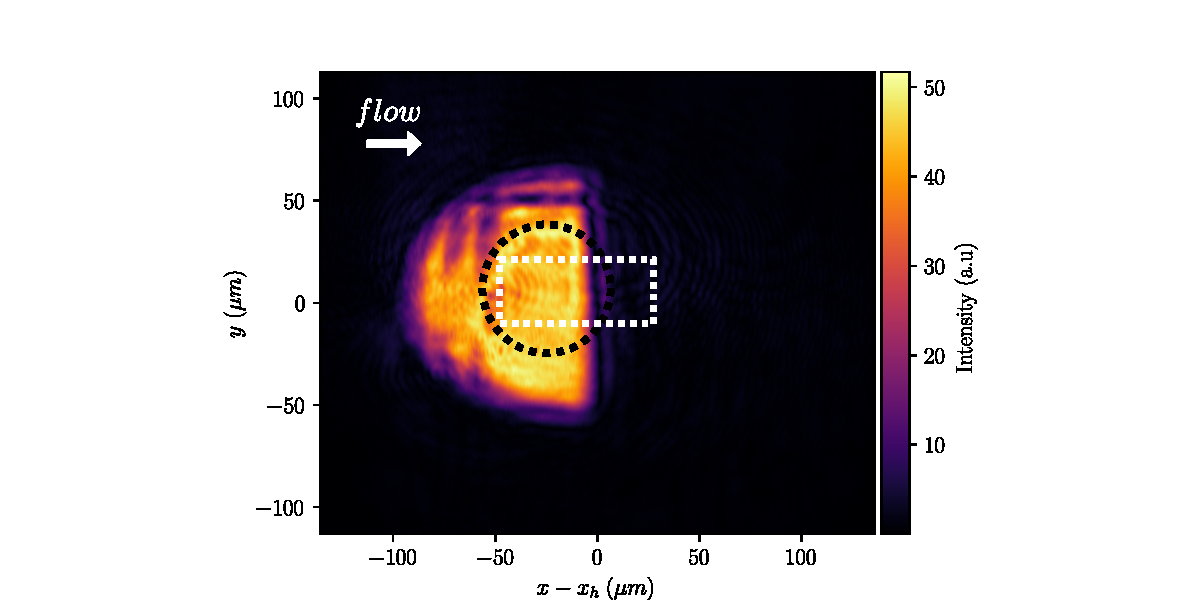
\includegraphics[width=1\textwidth]{chap_stimulated_hawking/fig/bh_density.pdf}
    \caption{\textbf{a)} Real space image of a transcritical flow of polaritons with detuning $\delta(0)=\SI{48}{\giga\hertz}$. The pump is shinned only 
    in the upstream region with wavevector $k_p=\SI{0.02}{\per \micro \meter}$.
    The downstream region is made of polaritons propagating ballistically. The black dashed circle represent the location of the injected probe while the white dashed rectangle represent the region 
    of interest (ROI) for the density and velocity profiles. }
    \label{fig:bh_density}
\end{figure}

As shown on the corresponding intensity and velocity profiles [see \autoref{fig:bh_balistic}~\textbf{a)}], the downstream region exhibits an exponentially decaying density accompanied by an increasing flow velocity. 
This behavior naturally arises from the conservation of current, as described by the continuity equation ~\ref{eq:continuity}, in the absence of external pumping. More precisely, it can be shown that 
away from the pump spot in slowly varying region where the quantum pressure can be neglected, the Gross Pitaevskii equation takes the form of generalized Bernoulli equation for driven dissipative fluid. The wavefunction then takes the form \cite{carusotto_inhomogeneous_2008}: 

\begin{equation}
    \psi_0(x \gg x_h) = \sqrt{n_0}e^{-\frac{x}{l_d}}e^{i k_{fluid}x},
\end{equation}
where $1/l_d=\gamlp/2v_g$ is the spatial decaying rate resulting from the product between the fluid group velocity $v_g =\hbar k_{fluid}/\mlp $ and the polariton lifetime $1/\gamlp$. The local wavevector of the polariton fluid $k_{fluid}$ is determined by the equation: 
\begin{equation} 
    \hbar \omp = \hbar \omlp + \frac{\hbar^2 k_{fluid}^2}{2m} + gn_0(x) + g_r n_r(x).
    \label{eq:bernoulli}
\end{equation}
Taking the low density limit $gn_0, g_rn_r \to 0$, the asymptotic value of $k_fluid$ is fixed by the detuning $\delta(0)$ in the pumped region as $k_d \coloneqq k_{fluid}(x \gg x_h) = \sqrt{2m\delta(0)}/\hbar$.
This evolution can also be intuitively understood through an optical analogy: photons propagating from the pumped region encounter a zone of lower polariton density, which corresponds to a higher effective refractive index. According to Snell-Descartes laws of refraction, the wavevectors of the photons are bent toward the normal of the interface, effectively resulting in an increase in the group velocity. 
The corresponding velocity profile measured by off axis interferometry is depicted in \autoref{fig:bh_balistic}~\textbf{b)}.  The horizon then forms
spontaneously due to the simultaneous increasment of the flow velocity and the decreasment of the speed of sound.

\bigskip


\textcolor{red}{\textbf{TODO : add the speed of sound measurement;}}
In this configuration the surface gravity is $\kappa\approx \SI{18}{\per \pico \second}$ which is two order of magnitude higher than what was obtained 
in the steepest horizon of the previous chapter. The price we pay for this enhancement is the appearance of oscillations in the fluid density and velocity profiles.
Indeed, since the pump is no longer present to fix the phase of the system and inject density, the fluid is more sensitive to fabrication defects in the microcavity each of them
acting as a scattering center.



\begin{figure}
    \centering
    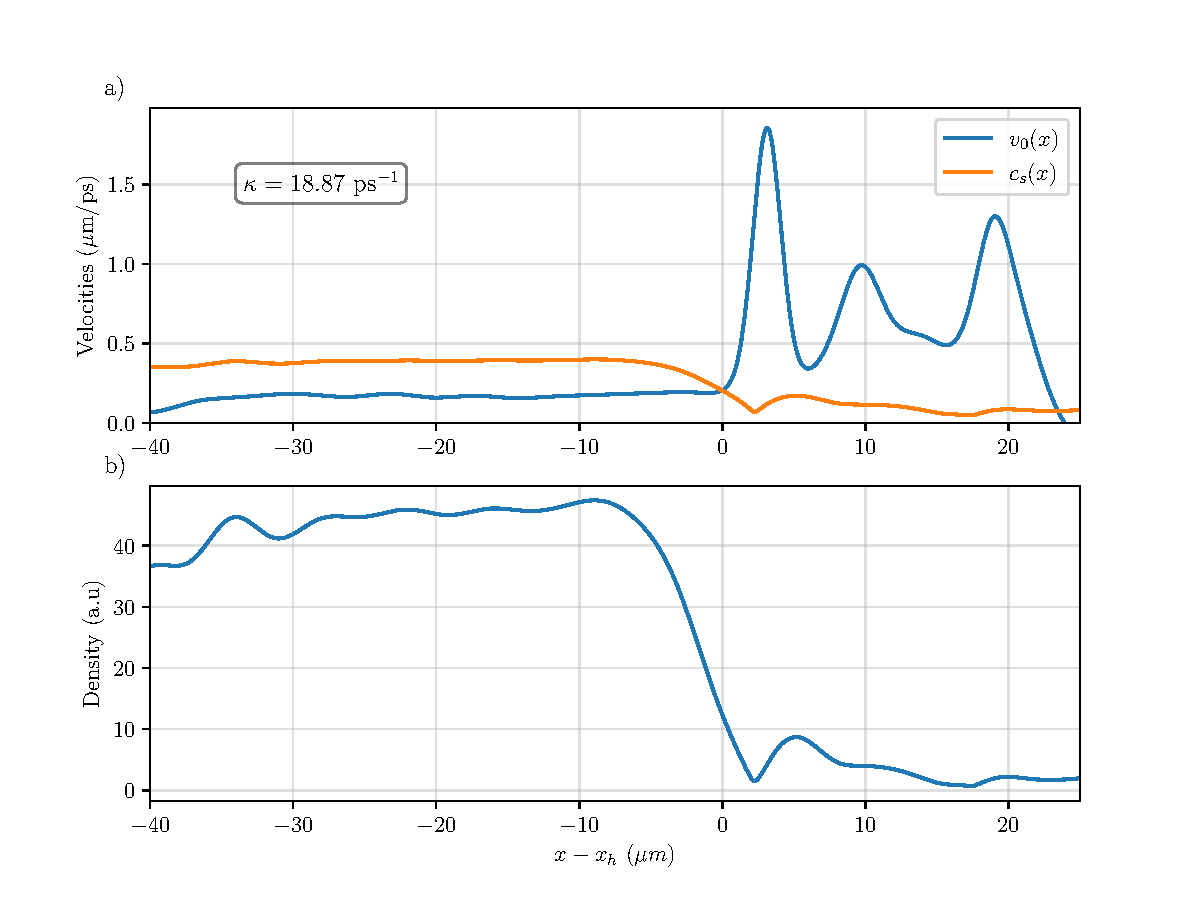
\includegraphics[width=1\textwidth]{chap_stimulated_hawking/fig/bh_balistic.pdf}
    \caption{\textbf{a) Density profile of the polariton fluid taken in the region of interest.} The profile is obtained by taking an
    average along the $y$-axis on the whole ROI represented by the white dashed rectangle of \autoref{fig:bh_density}. \textbf{b)} \textbf{Velocity profiles of the fluid in the ROI.} The blue curve corresponds to the velocity of the fluid obtained by off axis interferometry. The orange
    curve corresponds to $c_s=\sqrt{gn_0/\mlp}$ calibrated from the value of $gn_0$ fitted from the upstream Bogoliubov spectrum.}
    \label{fig:bh_balistic}
\end{figure}

\subsection{Measurement of the Bogoliubov spectrum}

In order to determine whether a detected signal originates from genuine scattering at the interface or from a spurious scattering event, we begin by characterizing the Bogoliubov excitation spectrum of the fluid in each region independently.
This is done by employing a technique mixing the high resolution pump probe spectroscopy detailed in the previous chapter and the interferometric technique described in the previous section.

\bigskip

First, the probe beam is centered in the upstream region close to the interface as represented by the black dashed circle in \autoref{fig:bh_density}~\textbf{a)}.
A sligth spatial overlap with the downstream region across the interface is voluntarily introduced to have acces to the spectrum of both regions on a single frequency scan as we will see later. To remain in 
the perturbative regime, the probe intensity is kept two orders of magnitude lower than the pump intensity.
Then, the whole field is superimposed with a collimated phase reference beam originating from the probe laser. As a rule of thumb, the diameter of the reference is 
increased to be three times larger than the diameter of the probe beam in order to have the flatest possible phase front.
 The angle difference between the two beams is set to obtain the best spatial frequency resolution as explained in \autoref{sec:phase_measurement}.


Secondly, the wavevector of the probe beam is tunned from $\SI{-1.0}{\per \micro \meter}$ to $\SI{1.0}{\per \micro \meter}$ by 60 steps of $\Delta k =\SI{0.046}{\per \micro \meter}$.
At each step, the probe frequency is scanned $\SI{130}{\giga \hertz}$ around the pump frequency. The main difference with the previous experiment arises in the detection scheme. Indeed, instead of modulating 
the probe intensity to latter isolate the signal by electronic filtering, we use the interferometric technique aforementioned. A single frequency scan consist 
in a series of 80 interferograms recorded on a CCD camera. A full dataset is then made of $80\times 60$ interferograms where each image has $2056\times 2464$ pixels encoded on 16 bits
for the best dynamical range. Obviously, compared to the $600$ hundreds points per energy scan available with the previous technique,
the present procedure suffer from a lack of frequency resolution. This being said, frequency resolution was never a limitation and this drawback
is largely compensated by the advantages of the interferometric technique. In particular, it allows to measure almost all the relevant observables in a single data set 
as we shall see now. 

\begin{figure}
    \centering
    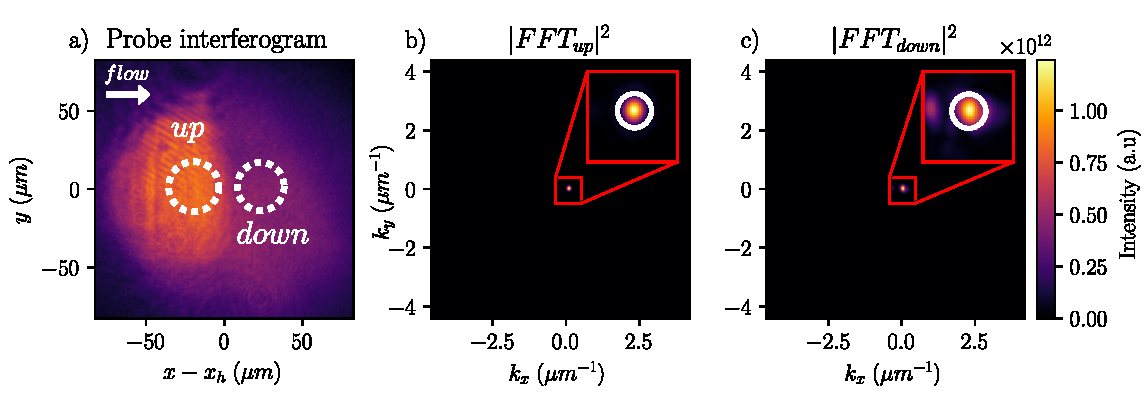
\includegraphics[width=1\textwidth]{chap_stimulated_hawking/fig/fft_bh_fluctu.pdf}
    \caption{\textbf{a) Probe interferogram.} The probe is located in the upstream region as in \autoref{fig:bh_density}. The white dashed circle represent the numerical mask applied to isolate each region.
    \textbf{b)} Shifted fourier transform of the masked interferogram of the upstream region. The red inset is a zoom on a $\SI{0.2}{\per \micro \meter}$ region around the probe spot where the solid white circle correspond to the numerical pinhole applied to isolate the probe signal.
    \textbf{c)} Shifted fourier transform of the masked interferogram of the downstream region. The red inset is a zoom on a $\SI{0.2}{\per \micro \meter}$ region around the probe spot where the solid white circle correspond to the numerical pinhole applied to isolate the probe signal.}
    \label{fig:fft_bh_fluctu}
\end{figure}

\textbf{Spectrum reconstruction.} For each interferogram, a Gaussian numerical mask of width \SI{40}{\micro \meter} is (see ~\ref{fig:bh_density}) applied either in the upstream or downstream region to spatially isolate the area of interest. A two-dimensional Fourier transform is then performed on the masked interferograms, yielding the fluctuation spectrum at the probe frequency within the selected region.
Initially, our objective is to extract the Bogoliubov dispersion relation in each region, which—as discussed in the previous chapter—can be inferred from the transmission spectrum of the probe across the sample. To this end, an additional numerical pinhole, centered on the probe wavevector and with a radius matched to the probe spot, is applied in the Fourier domain of the interferogram, as illustrated in \autoref{fig:fft_bh_fluctu}.
The integral over the masked fourier planes provides the transmission of the probe in the corresponding region.


In summary, for each probe configuration defined by the wavevector-frequency pair \((k_{in}, \omega_{in})\), this procedure yields the transmitted probe intensity \(I_{u,d}(k_{in}, \omega_{in})\) in both upstream and downstream regions.
At this stage, the reason for positioning the probe beam to slightly overlap with the downstream region becomes evident : it allows for the direct excitation of Bogoliubov modes with minimal influence from the interface. This is essential for benchmarking the dispersion relation of modes transmitted from upstream, and for confirming that they coincide with those excited locally in the downstream region.
By repeating this procedure for all probe configurations, we obtain the Bogoliubov dispersion in each region, as shown in \autoref{fig:bh_spectrum}.  As anticipated, only the normal branch is accessible via direct excitation. This is not a limitation but rather a deliberate feature of the method, which was specifically chosen for its ability to isolate the positive frequency signals. 
Besides, knowledge of the normal branch alone is sufficient to reconstruct the full Bogoliubov spectrum, as its structure is inherently symmetric. Moreover, the existence of the ghost branch, particularly its positive-frequency domain which is essential for the Hawking effect in the supercritical regime, was established in the previous chapter. Consequently, we will not try to measure it in the present work.
\begin{figure}
    \centering
    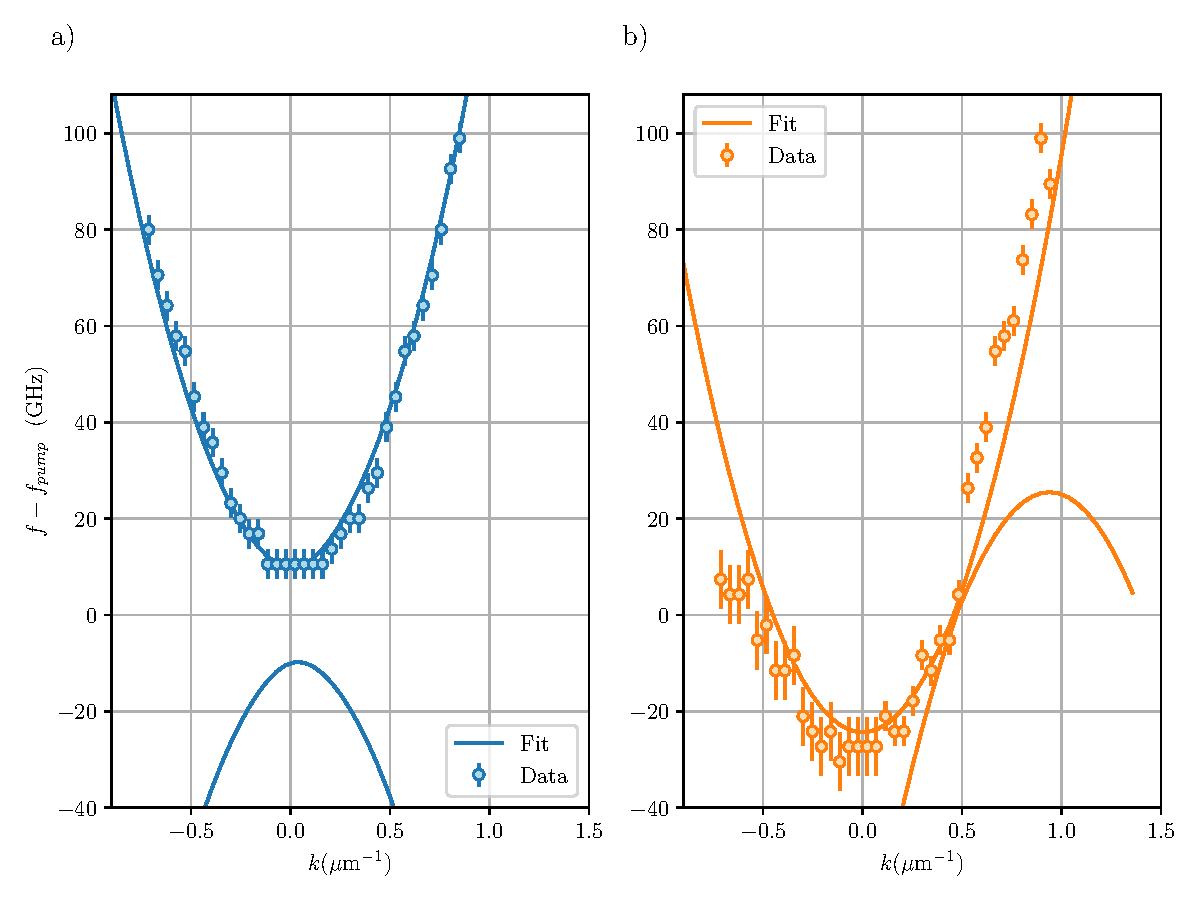
\includegraphics[width=1\textwidth]{chap_stimulated_hawking/fig/fit_bogo.pdf}
    \caption{\textbf{a)-b)} \textbf{Upstream-Downstream Bogoliubov spectrum}. The scattered points correspond to the maxima of the transmission spectrum of the probe in the upstream-downstream region. The blue-orange solid 
    line is the analytical bogoliubov dispersion plotted with the experimental parameters and the non linear interactions $gn_0$ obtained from
    the fit of the data with the normal bogoliubov branch. The upstream region fit gives $gn_0 =9.6 \pm \SI{0.1}{\giga \hertz}$ while in the downstream we obtain $gn_0=1.2\pm \SI{0.01}{\giga \hertz}$.
    The vertical errorbars are mainly originating from the frequency resolution of the measurement while the horizontal uncertainties are due to the probe extension in momentum space $\sigma_k =\SI{0.04}{\per \micro \meter}$.}
    \label{fig:fit_bogo}
\end{figure}
\bigskip 

The upstream spectrum shown in \autoref{fig:fit_bogo}~\textbf{a)} exhibits a gap and a slight doppler shift consistent with the pump wavevector in the pumped upstream region $k_p=\SI{0.023}{\per \micro \meter}$. The data points are fitted with the Bogoliubov dispersion relation \ref{eq:bogo_lab_frame} where $gn_0$ is the only fitting paramterers and the dark reservoir
is handled the same way as in the previous chapter. 
We obtain $gn_0=9.6\pm\SI{0.1}{\giga \hertz}$ and find a good agreement of the model with the experimental points. The downstream spectrum shown in \textbf{b)} possess negative frequency modes which is typical of a supercritical flow.
As explained earlier, the absence of pumping imposes the condition \ref{eq:bernoulli} that can be recast in the form $\delta(k_{fluid})=gn_0+g_rn_r$. It is the counterpart of the turning point condition in the pumped region implying that the Bogoliubov spectrum is expected to be linear far from the interface :

\begin{equation}
    \omega_B(k) = v_d(k-k_d) \pm \sqrt{\dfrac{\hbar (k-k_d)^2}{2\mlp} \left({\dfrac{\hbar (k-k_d)^2}{2\mlp}} + g n_0 \right)},
\end{equation}
where $v_d = \hbar k_d/\mlp$ is the asymptotic velocity of the fluid measured by off axis inteferometry. The fit gives $gn_0=\SI{1.2 \pm 0.01}{\giga \hertz}$. As visible, the agreement is not as good as in the upstream region. 
This is due to the fact that in the unpumped region, the fluid is not homogeneous anymore close to the interface as shown in \autoref{fig:bh_balistic} \textbf{b)}. Homogeneity,
is recovered far from the interface where the density is low enough. But whenever this condition is satisfied, there is no fluid left to probe.  Consequently, the signal measured mainly comes from the transcient region where looking for the bogoliubov modes as plane waves is already an approximation.
to obtain a beter agreement, a complete diagonalization of the Bogoliubov matrix around the steady state would be necessary in this region. However, this is not the goal of this work and the supercritical feature we are interested in
remain robust against this approximation.
This two measurements prove together the presence of an analogue horizon in between the two regions Now that the spectrum of collective excitation is known on both side of the 
interface. Let us now turn to the measurement of the scattering matrix.

\subsection{Measurement of the scattering matrix}
\label{sec:scattering_matrix}

\subsubsection{Detection of the scattered modes}

We analyze the emergence of transmitted or reflected modes resulting from an incoming perturbation propagating toward the horizon. 
We focus on the scattering of the \( u_{in}(k) \) modes. 
From the maxima of the upstream Bogoliubov spectrum, we select the set of configurations \((k, \omega)\) where the probe is exciting upstream modes with positive group velocity, i.e., \(\partial\omega/\partial k > 0\). 
For each configuration, we compute the Fourier transform of the probe field in both upstream and downstream regions, following the same separation procedure employed for the Bogoliubov spectrum reconstruction. 
In contrast to the earlier analysis, we now apply a numerical anti-pinhole to suppress the intense contribution of the \( u_{in} \) mode at the probe position. A peak-detection algorithm is then used to identify the positions of the scattered modes in the Fourier plane and to extract their corresponding wavevectors.
Each identified wavevector is compared with the Bogoliubov spectrum to confirm its physical relevance and to rule out spurious scattering events. This process is systematically repeated for all configurations associated with \( u_{in} \). The resulting scattering data are summarized in \autoref{fig:fit_bogo_RT} \textbf{a)}. As observed, the modes detected both in the upstream and dowstream regions 
are in good agreement with their respective Bogoliubov relations.

\begin{figure}
    \centering
    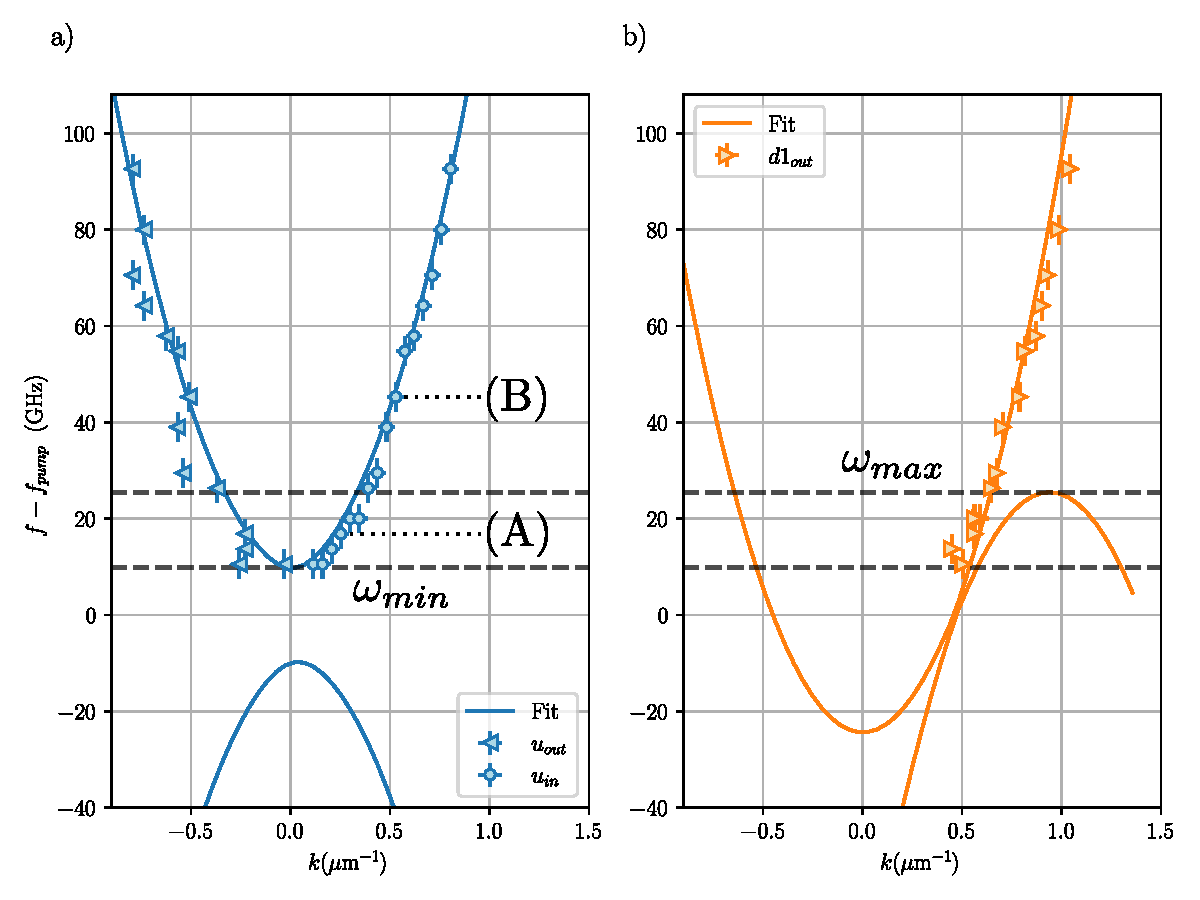
\includegraphics[width=1\textwidth]{chap_stimulated_hawking/fig/fit_bogo_RT.pdf}
    \caption{\textbf{a) Measurement of the reflected modes $u_{out}$} The $u_{in}$ modes excited by the probe are represented by the blue dots. The errorbars are the same than in \autoref{fig:fit_bogo}. For each $u_{in}$ mode
    the wavevector of the maximum detected in the upstream region is represented by the blue left oriented triangle. The errorbars are the same than for the $u_{in}$ modes with an additionnal contribution on the steeming from our momentum space resolution $\Delta=\SI{0.027}{\per \micro \meter}$ during the peak detection algorithm. The blue solid line
    is the fit of the upstream Bogoliubov dispersion obtained in \autoref{fig:fit_bogo} \textbf{a)} The black dashed lines defines the frequency range 
    at which negative-positive energy mixing is possible. 
    \textbf{b) Measurement of the transmitted modes.} The wavevector of the maximum detected in the downstream region is represented by the orange right oriented triangle. The errorbars are the same than in \textbf{a)}. 
    The orange solid line is the fit of the downstream Bogoliubov dispersion obtained in \autoref{fig:fit_bogo} \textbf{b)}. }
    \label{fig:fit_bogo_RT}
\end{figure}

This measurement demonstrates that the interface scatters the incoming mode as expected from the Bogoliubov theory. However, $d2_{out}$ is not detected in the downstream region. This is due to its negative norm stating the major part of the mode amplitude is on the conjugted branch.
Indeed, in the bogoliubov basis the excited $d2_{out}$ mode is written as :
\begin{equation}
    \begin{pmatrix}
        u_{k_{d2}^{out}} \\
        v_{k_{d2}^{out}}
    \end{pmatrix}e^{-i\omega_{pr}t}=
    \begin{pmatrix}
    U_{k_{d2}^{out}} \\
    V_{k_{d2}^{out}}
    \end{pmatrix}e^{ik_{d2}^{out}x}e^{-i\omega_{pr}t}, 
\end{equation}
where $\omega_{pr}$ is the probe frequency. According to ~\ref{eq:fluctuation_order_parameter} the corresponding fluctuation of the order parameter ie the physical quantity experimentally accessible, is :
\begin{equation}
    \delta\psi_{{d2}^{out}}(x,t)= U_{k_{d2}^{out}}e^{ik_{d2}^{out}x}e^{-i\omega_{pr}t}+V_{k_{d2}^{out}}^*e^{-ik_{d2}^{out}x}e^{i\omega_{pr}t}.
    \label{eq:order_param_d2_out}
\end{equation}
Due to its negative norm the bogoliubov amplitudes are such as $\int |U_{k_{d2}^{out}}|^2-|V_{k_{d2}^{out}}|^2=-1$ meaning that  $|V_{k_{d2}^{out}}|^2$ is significantly greater than $|U_{k_{d2}^{out}}|^2$. 
Consequently, its larger amplitude is at opposite frequency and wavevector, namely, in the $d2_{out}^*$ mode on the normal branch. This explains why the interferometric technique, which 
can detect only modes at the probe frequency fails to detect the weak amplitude of the $d2_{out}$ mode. To measure it, we use an imaging spectrometer Princeton Instruments SpectraPro SP-2750 mounted with a 1200 lines/mm grating together with a high sensitive CCD camera Teledyne PIXIS 1024. By 
imaging the Fourier plane of the entire field on the entrance slit of the spectrometer it is possible to directly obtain the spectrum of the fluid including both the pump and the probe contributions.
As the pump is generally two orders of magnitude brighter than the probe, it quickly saturates the camera sensor preventing to detect weak probe signals. To overcome this issue,
the pump is filtered out with a rasor blade placed in the real space of the field before the spectrometer. The blade is positioned in order to block the bright upstream region while letting the weak downstream region pass through.
This allows to set a long exposure time without being blinded by the pump. A typical spectrum taken with a 4 seconds exposure time is shown in \autoref{fig:bh_spectrum}~\textbf{a)}. By superimposing the image with the downstream Bogoliubov dispersion obtained earlier, the different modes are identified and their positions 
are represented by colored dashed circles. Remarkably, an intensity peak is observed at the $d2_{out}^*$ mode, as visible on the vertical cut \textbf{b)}. It is worth noticing that this peak disappears when the probe 
is exciting an input mode outside of the negative-positive energy mixing region. Finally, an additionnal peak is observed at twice the probe frequency. We interpret it 
as the result of a four wave mixing process where two $d1_{out}$ polaritons scatters into a pump mode polariton and a higher energy mode :
\begin{equation}
    \begin{aligned}
    (\omega_{pr}, \omega_{pr}) &\to (0, 2\omega_{pr}) \\
    (k_{d1}^{out}, k_{d1}^{out}) &\to (k_{d1}^{out}-\Delta k,k_{d1}^{out}+\Delta k),
    \end{aligned}
    \label{eq:higher_order_four_wave_mixing}
\end{equation}
where $\Delta k= k_{d1}^{out}-k_d$ is the wavevector mismatch between the pump in the downstream region and the $d1_{out}$ mode. This process is a bosonic stimulation triggered by the high 
occupation of the pump state and is particularly efficient because of the linearity of the Bogoliubov spectrum provinding a great phase matching 


\begin{figure}
    \centering
    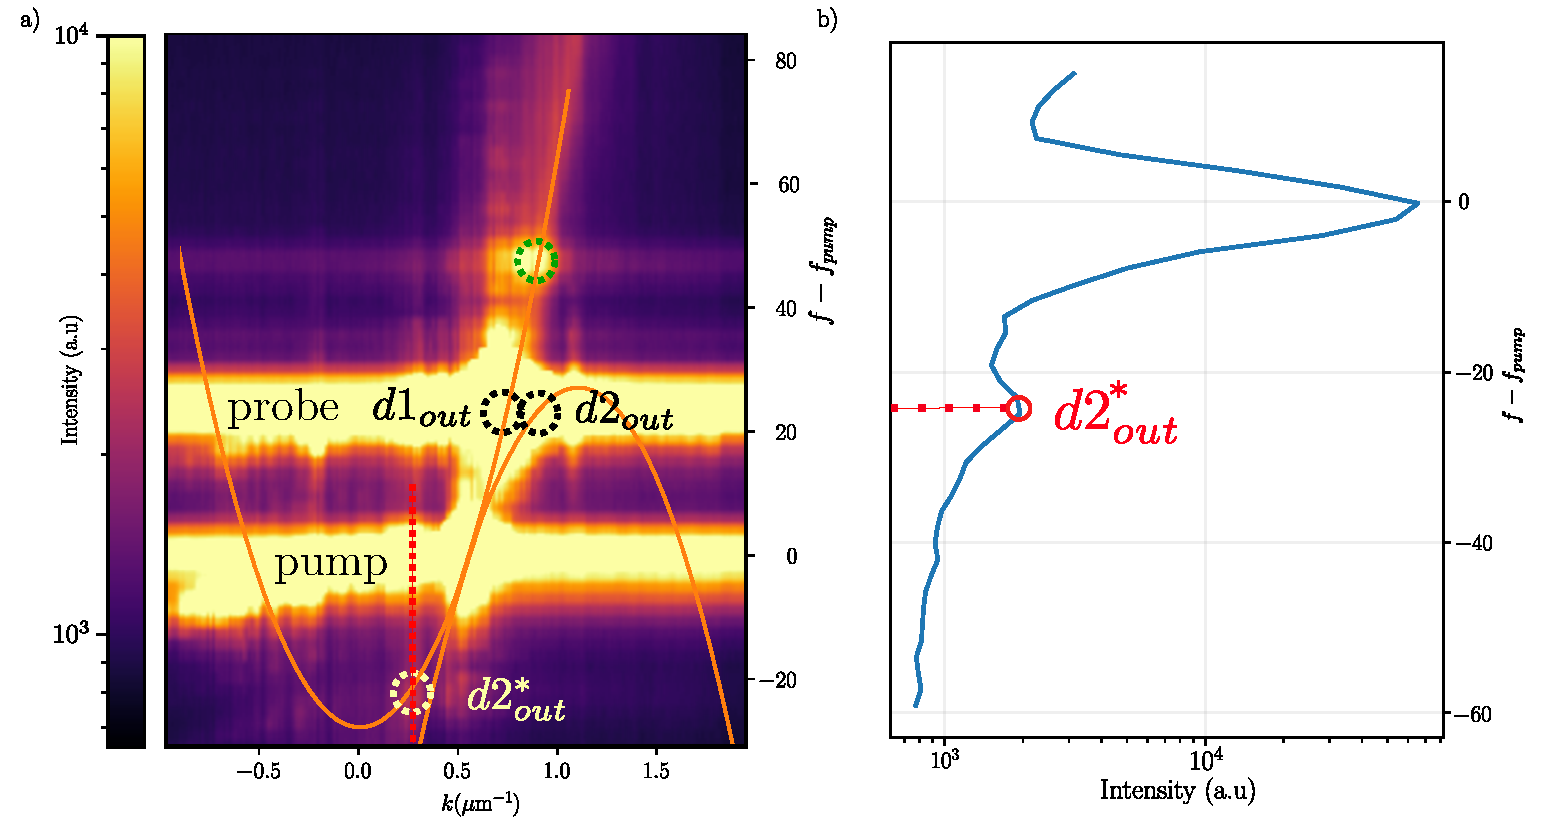
\includegraphics[width=0.8\textwidth]{chap_stimulated_hawking/fig/disp_supersonic_spectro.pdf}
    \caption{\textbf{a) Spectrum of the downstream region of the flui.} The spectrum is taken by integrating the whole downstream region of the fluid during 4 seconds
    with an imaging spectrometer. The orange solid line represent the fit of the Bogoliubov dispersion relation obtained in \autoref{fig:fit_bogo} \textbf{b)}. The dashed black line is the expected location of the $d2_{out}$ mode.
    The red dashed circle is the $d2_{out}^*$ mode, conjugated of $d2_{out}$. 
    \textbf{b) Vertical cut of the $d2_{out}^*$ mode.} The intense peak on the right corresponds to the remaining pump contribution. The red dashed vertical line locates the $d2_{out}^*$ mode.}
    \label{fig:spectrum_spectro}
\end{figure}
\bigskip

\subsection{A signature of amplification}
As explained in \autoref{chap:AG_theory}, if the incoming mode is modeled as a coherent state $\ket{\alpha_{in}}$ with amplitude $\alpha_{in}$, it is possible to compute the average number of quanta in each output mode.

\subsubsection{Input and output modes descrimination}
Consider the perturbation field $\delta\psi$ when the probe is exciting a given input mode in the upstream region. In a first approch we restrict our description to 
what is experimentally accesible with our interfometric method, namely, the field at the probe energy only. In a very general way, the wavefunction can be decomposed as follows:

\begin{equation}
    \begin{aligned}
    \delta\psi(x,t) &= \delta \psi_{in}(x,t)+\delta \psi_{res}(x,t) \\
    &= \delta \psi_{in}(x,t) + \delta \psi_{scat}(x,t) + \delta \psi_{err}(x,t).
    \end{aligned}
\label{eq:scat_decomp}
\end{equation}
where $\delta \psi_{in}$ is the ideal incoming mode and $\delta \psi_{res}$ is the residual field. The latter is made of all the other modes that are not in the $in$ mode. The term $\psi_{scat}$ represents all the scaterings that may 
occur in the fluid. In particular, it contains the outgoing modes $u_{out}$, $d_1^{out}$ and $d_2^{out}$ that are the result of the scattering process. Furthermore, the residual field also accounts for deviations
of the injected probe beam in the cavity from the perfect gaussian beam defined by $\delta \psi(x,t)$. This contribution $\delta \psi_{err}(x,t)$ is purely optical and can be thought as a biais when $\psi_{in}$ is extracted from the true probe beam as we shall see now.

\bigskip

\textbf{Input mode.} The safest way to define the input while minimizing the biais is to perform the fourier transform of the perturbation field and 
use modal decomposition. As in the previous section we first detect the amplitude peak of the injected mode that is the major contribution in the fourier space. Cuts along both axis of the detected peak are shown in \autoref{fig:fit_input_mode} \textbf{a)} and \textbf{b)}.
 A few comments can already be done. First, one can notice that the 
peak is centered at $\kvec=(k^{in}_x, k^{in}_y) = (0.23 , 0.0)$ reflecting the positive group velocity of the injected mode. On the other hand, the peak is not perfectly
symmetric and is sligthly deformed in the $k_x$ direction. It's worth stressing that it is hard to determine whether this elongated shape already contains
information about the scattering process or if it's a broadening resulting from the fluid motion only. To overcome this issue,
we use the cut of the peak in the $k_y$ direction using that the fluid is still translationnaly invariant in this direction as explained in \autoref{chap:AG_theory}.
The $y$ cut is then fitted with a 1D gaussian amplitude of the  form $f(k_y)=\mathrm{A}\mathrm{exp}(-(k_y-k_y^0)^2/(2\sigma^2))$ and the result is shown in \textbf{a)}.
As visible, the fit matches well the data. The values of the amplitude $\mathrm{A}$ and the width $\sigma$ are then used to define a 2D gaussian function with the same amplitude and width, centered 
at $\kvec$ : 

\begin{equation}
    \mathrm{A_{fit}}(k_x,k_y) = \mathrm{A} \mathrm{exp}(-\frac{(k_x-k_x^0)^2}{2\sigma^2}-\frac{(k_y-k_y^0)^2}{2\sigma^2}).
    \label{eq:gaussian_amp} 
\end{equation}
To end the definition of the input mode complex field, we need to provide it with a phase. To do so, we look at the phase of the $\delta \tilde{\psi}$ 
in the vicinity of the peak. Close to the maximum amplitude, the phase is well defined and is approximated by a planar surface by 
fitting the signal with a function of the form $\theta_{fit}(k_x, k_y)=ak_x+bk_y+c$ where $a$, $b$ and $c$ are the fitting parameters.
In fact encode the position of the in mode in real space and could also be determined by computing the barycenter
of the probe intensity in real space. This fitting procedure is equivalent to neglect any curvature 
in the mode wavefront or in other words to assume that the mode is a plane wave. Of course, fluctuations 
around this ideal phase are expected and may contains information about the scattering process. To take this into account we perform a last step 
consisting in projecting the overall field $\delta \tilde{\psi}$ on the ideal input mode we just defined ie $\delta \tilde{\psi}_{\mathrm{fit}}(\kvec)= \mathrm{A_{fit}}(\kvec)\mathrm{exp}(i\theta_{\mathrm{fit}}(\kvec))$.
The resulting field is then given by : 

\begin{equation}
    \delta \tilde{\psi}_{in} = \bra{\delta \tilde{\psi}_{\mathrm{fit}}}\ket{\delta \tilde{\psi}} \delta \tilde{\psi}_{\mathrm{fit}}. 
    \label{eq:input_mode_scalar_product}
\end{equation}

\bigskip 

\textbf{Residual field.} From the above expression, we are able to define the residual field as the difference between the injected mode and the overall field $\delta \tilde{\psi}_{res} = \delta \tilde{\psi}-\delta \tilde{\psi}_{in}$. 
Note that the way $\delta \tilde{\psi}_{in}$ is built through a scalar product ensures that the residual field is orthogonal to the $in$ mode provided $\delta \tilde{\psi}_{fit}$ is normalized :

\begin{equation}
    \begin{aligned}
    \bra{\delta \tilde{\psi}_{in}}\ket{\delta \tilde{\psi}_{res}} &=\bra{\delta \tilde{\psi}_{\mathrm{fit}}}\ket{\delta \tilde{\psi}} \left(\bra{\delta \tilde{\psi}_{\mathrm{fit}}}\ket{\delta \tilde{\psi}} - \bra{\delta \tilde{\psi}_{\mathrm{fit}}}\ket{\delta \tilde{\psi}_{in}}\right)\\
    &= \bra{\delta \tilde{\psi}_{\mathrm{fit}}}\ket{\delta \tilde{\psi}} \left(\bra{\delta \tilde{\psi}_{\mathrm{fit}}}\ket{\delta \tilde{\psi}}-\bra{\delta \tilde{\psi}_{\mathrm{fit}}}\ket{\delta \tilde{\psi}_{\mathrm{fit}}}\bra{\delta \tilde{\psi}_{\mathrm{fit}}}\ket{\delta \tilde{\psi}}\right)\\
    &=0.
    \end{aligned}
\end{equation}

In this manner, the basis chosen for our description is as close as possible to the Bogoliubov plane wave basis explicited in \autoref{chap:AG_theory}. This is a strong assumption 
that will be discussed in the next section. Now that the differents fields are defined, 

So far, the field description was done on the full space instead of a local analysis in the interface vicinity. Their respective intensities are displayed in \autoref{fig:fit_input_mode} \textbf{c)} and \textbf{d)}.

\begin{figure}
    \centering
    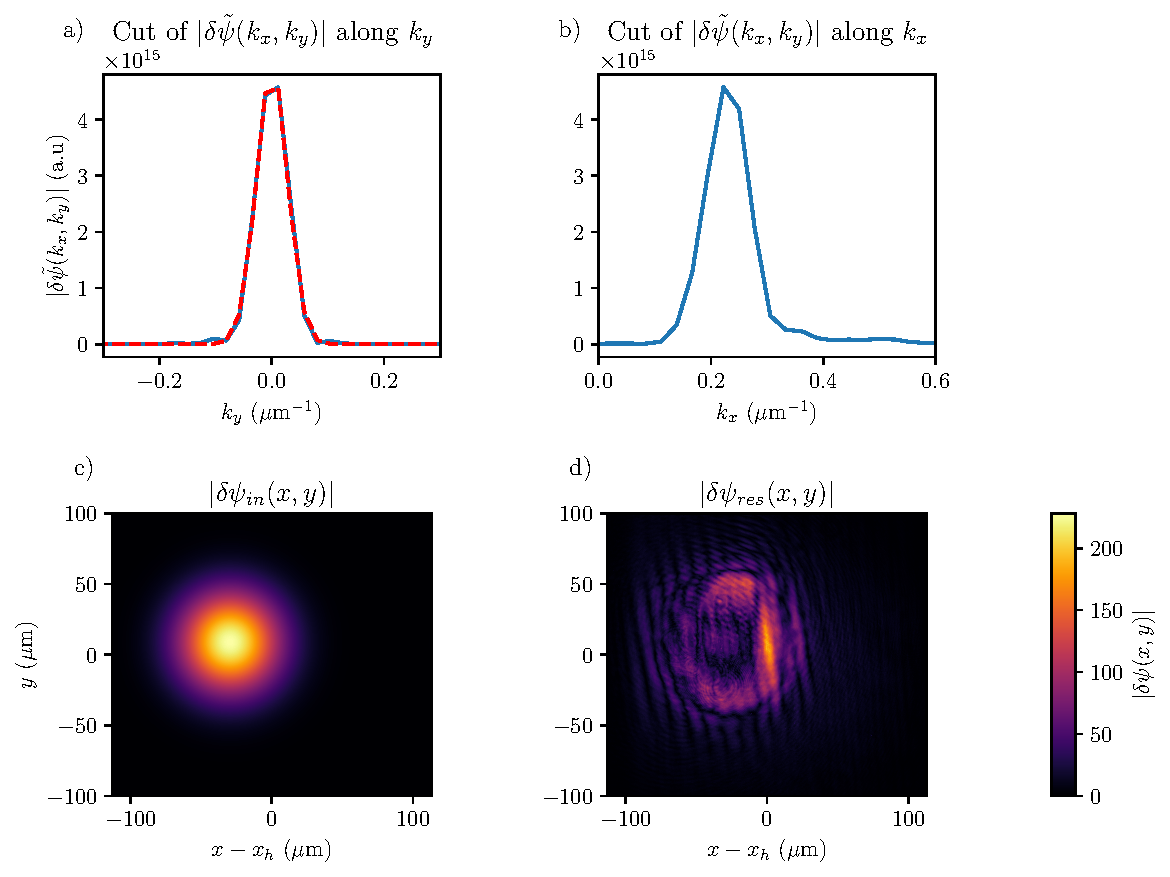
\includegraphics[width=1\textwidth]{chap_stimulated_hawking/fig/fit_input_mode.pdf}
    \caption{\textbf{a) Cut of the injected mode in the $k_y$ direction.} The blue curve is the data and the red dashed curve is the gaussian fit. The model has a R-squared value of 0.98. The amplitude $A$ and width $\sigma$ are extracted from the fit. 
    \textbf{b) Cut of the injected mode in the $k_x$ direction.}
    \textbf{c) Reconstructed input mode in real space.} Obtained by applying the inverse fourier transform to $\delta \psi_{in}(k_x,k_y)$.
    \textbf{d) Reconstructed residual field in real space.} Obtained by applying the inverse fourier transform to $\delta \psi_{res}(k_x,k_y)$.}
    \label{fig:fit_input_mode}
\end{figure}